% The variational quantum eigensolver as one picture (notebook 42a, Section 1).
% Left: the parametrised circuit U(theta) acting on |0>^N.  Middle: H = sum_j c_j P_j split into commuting groups,
% each group measured after its own basis rotation B_g.  Right: the cost C(theta) = sum_j c_j <P_j>.
% Bottom: the classical update theta <- theta - eta grad C, fed back into the circuit.
\documentclass[tikz,border=6pt]{standalone}
\usepackage{amsmath,amssymb,bm}
\usetikzlibrary{arrows.meta,positioning,calc,fit}
\newcommand{\ket}[1]{\lvert #1\rangle}
\begin{document}
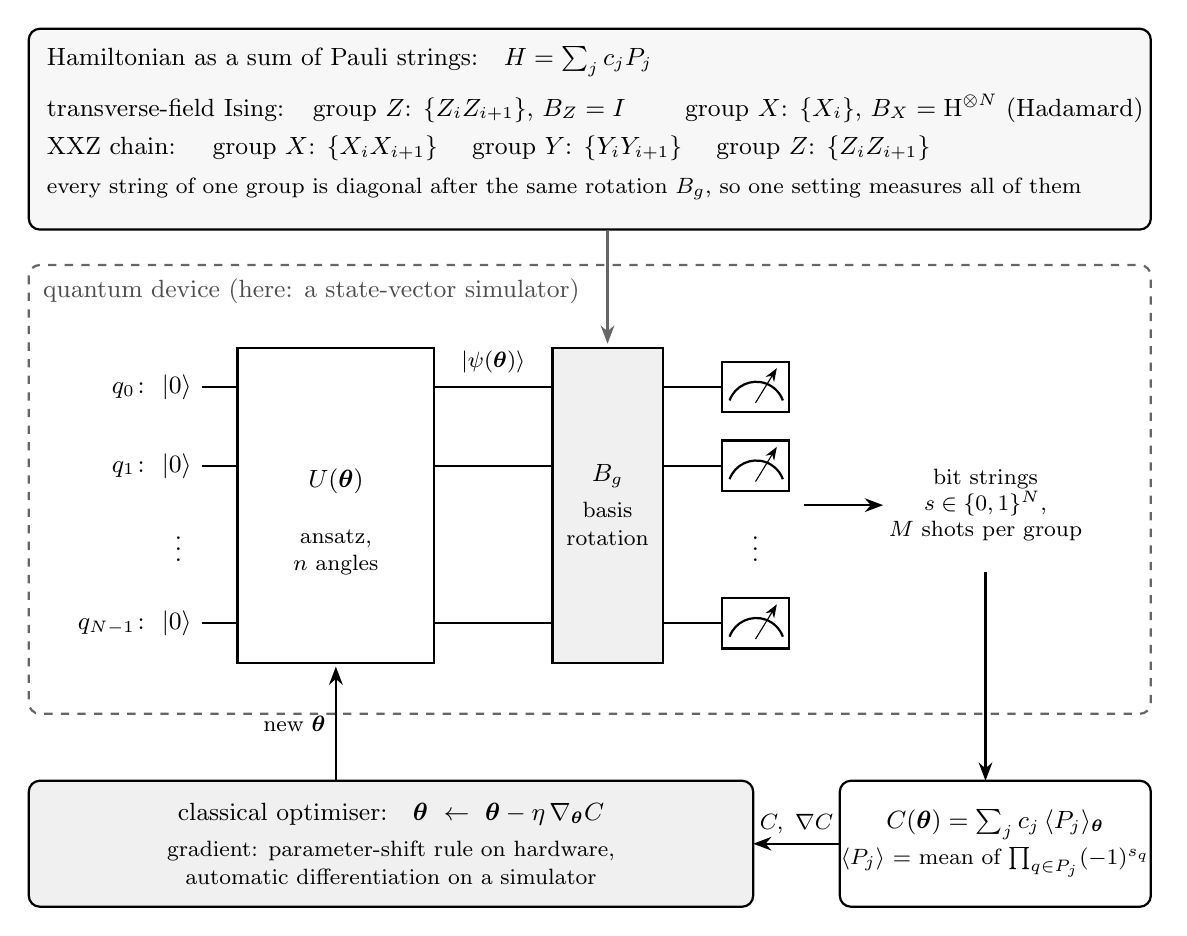
\begin{tikzpicture}[thick, >=Stealth, font=\small]
  % ---------------------------------------------------------------- quantum part
  \draw[dashed, rounded corners, black!60] (-1.9,1.55) rectangle (12.35,-4.15);
  \node[anchor=north west, black!70] at (-1.85,1.5) {quantum device (here: a state-vector simulator)};
  \foreach \y/\lab in {0/{q_0}, -1/{q_1}, -3/{q_{N-1}}} {
    \node[anchor=east] at (0.3,\y) {$\lab\colon\ \ket{0}$};
    \draw (0.3,\y) -- (6.9,\y);
  }
  \node at (0.0,-1.95) {$\vdots$};
  % circuit U(theta)
  \draw[fill=white] (0.75,0.5) rectangle (3.25,-3.5);
  \node at (2.0,-1.2) {$U(\boldsymbol\theta)$};
  \node[align=center, font=\footnotesize] at (2.0,-2.1) {ansatz,\\ $n$ angles};
  \node[above, font=\footnotesize] at (4.0,0.05) {$\ket{\psi(\boldsymbol\theta)}$};
  % basis rotation for group g
  \draw[fill=black!6] (4.75,0.5) rectangle (6.15,-3.5);
  \node[align=center] at (5.45,-1.5) {$B_g$\\[2pt]{\footnotesize basis}\\[-1pt]{\footnotesize rotation}};
  % meters
  \foreach \y in {0,-1,-3} {
    \draw[fill=white] (6.9,\y+0.32) rectangle (7.75,\y-0.32);
    \draw (7.0,\y-0.17) arc (160:20:0.36);
    \draw[->, thin] (7.33,\y-0.2) -- (7.6,\y+0.24);
  }
  \node at (7.33,-1.95) {$\vdots$};
  \node[align=center, font=\footnotesize] at (10.25,-1.5) {bit strings\\$s\in\{0,1\}^N$,\\ $M$ shots per group};
  \draw[->] (7.95,-1.5) -- (8.95,-1.5);
  % --------------------------------------------------------------- Hamiltonian box
  \draw[fill=black!3, rounded corners] (-1.9,4.55) rectangle (12.35,2.0);
  \node[anchor=north west] at (-1.8,4.45) {Hamiltonian as a sum of Pauli strings:\quad $H=\sum_j c_j P_j$};
  \node[anchor=north west, align=left] at (-1.8,3.85) {%
    transverse-field Ising: \ \ group $Z$: $\{Z_iZ_{i+1}\}$, $B_Z=I$ \qquad
    group $X$: $\{X_i\}$, $B_X=\mathrm{H}^{\otimes N}$ (Hadamard)\\[3pt]
    XXZ chain: \quad group $X$: $\{X_iX_{i+1}\}$ \quad group $Y$: $\{Y_iY_{i+1}\}$ \quad group $Z$: $\{Z_iZ_{i+1}\}$\\[3pt]
    {\footnotesize every string of one group is diagonal after the same rotation $B_g$, so one setting measures all of them}};
  \draw[->, black!60] (5.45,2.0) -- (5.45,0.55);
  % --------------------------------------------------------------- cost
  \draw[fill=white, rounded corners] (8.4,-5.0) rectangle (12.35,-6.6);
  \node[align=center] at (10.375,-5.8) {$C(\boldsymbol\theta)=\sum_j c_j\,\langle P_j\rangle_{\boldsymbol\theta}$\\[2pt]{\footnotesize $\langle P_j\rangle$ = mean of $\prod_{q\in P_j}(-1)^{s_q}$}};
  \draw[->] (10.25,-2.35) -- (10.25,-5.0);
  % --------------------------------------------------------------- optimiser
  \draw[fill=black!6, rounded corners] (-1.9,-5.0) rectangle (7.3,-6.6);
  \node[align=center] at (2.7,-5.8) {classical optimiser:\quad $\boldsymbol\theta\ \leftarrow\ \boldsymbol\theta-\eta\,\nabla_{\boldsymbol\theta}C$\\[2pt]
    {\footnotesize gradient: parameter-shift rule on hardware,}\\[-1pt]{\footnotesize automatic differentiation on a simulator}};
  \draw[->] (8.4,-5.8) -- node[above, font=\footnotesize]{$C,\ \nabla C$} (7.3,-5.8);
  \draw[->] (2.0,-5.0) -- node[left, font=\footnotesize]{new $\boldsymbol\theta$} (2.0,-3.55);
\end{tikzpicture}
\end{document}
